\documentclass[12pt]{article}

\usepackage{amsmath}
\usepackage{amssymb}
\usepackage{graphicx}
\usepackage{algorithm}% http://ctan.org/pkg/algorithms
\usepackage{algpseudocode}% http://ctan.org/pkg/algorithmicx
\usepackage{framed} % or, "mdframed"
\usepackage[framed]{ntheorem}
\usepackage{listings}
\usepackage{color}
\usepackage[usenames,dvipsnames,svgnames,table]{xcolor}

\newframedtheorem{frm-thm}{Lemma}

\usepackage[scale=1.0, left=1.0cm, right=1.0cm, top=1.865cm, bottom=0.865cm]{geometry}
\DeclareMathOperator*{\argmin}{arg\,min}

\definecolor{dkgreen}{rgb}{0,0.6,0}
\definecolor{dred}{rgb}{0.545,0,0}
\definecolor{dblue}{rgb}{0,0,0.545}
\definecolor{lgrey}{rgb}{0.9,0.9,0.9}
\definecolor{gray}{rgb}{0.4,0.4,0.4}
\definecolor{darkblue}{rgb}{0.0,0.0,0.6}
\lstset{ 
      backgroundcolor=\color{lgrey},  
      basicstyle=\footnotesize \ttfamily \color{black} \bfseries,   
      breakatwhitespace=false,       
      breaklines=true,               
      captionpos=b,                   
      commentstyle=\color{dkgreen},   
      deletekeywords={...},          
      escapeinside={\%*}{*)},                  
      frame=single,                  
      keywordstyle=\color{purple},  
      morekeywords={BRIEFDescriptorConfig,string,TiXmlNode,DetectorDescriptorConfigContainer,istringstream,cerr,exit}, 
      identifierstyle=\color{black},
      stringstyle=\color{blue},      
      language=C,                
      numbers=right,                 
      numbersep=5pt,                  
      numberstyle=\tiny\color{black}, 
      rulecolor=\color{black},        
      showspaces=false,               
      showstringspaces=false,        
      showtabs=false,                
      stepnumber=1,                   
      tabsize=5,                     
      title=\lstname,                 
    }


\pagestyle{myheadings}
\markright{CSE 260, Assignment 1 \hfill Andrew Conegliano, Matthias Springer\hfill}

\begin{document}

\title{Double-precision General Matrix Multiply (DGEMM)  \\ \vspace{2 mm} {\large Parallel Computation (CSE 260), Assignment 1}}
%\subtitle{Parallel Computation (CSE 260), Assignment 1}
\date{\today}
\author{Andrew Conegliano \and Matthias Springer}
\maketitle

\section{Introduction}

\subsection{Assumptions}
\begin{itemize}
	\item All matrices are square matrices.
	\item All matrices consist of double-precision floating point values (64-bit doubles).
\end{itemize}

\subsection{Notation}
In this work, we use the following notation and variable names.
\begin{itemize}
	\item $n$ is the size of one dimension of the matrices involved. I.e., every matrix has $n^2$ values.
	\item When referring to matrices, $A$ and $B$ denote the source matrices and $C$ denotes the target matrix, i.e. $AB = C$.
	\item $b_i$, $b_j$ and $b_k$ denote the block size for each \emph{dimension} $i$, $j$, and $k$, respectively\footnote{We tried multiple levels of blocking and it is evident from the context which level of blocking we are refering to.}.
\end{itemize}

\section{Runtime Environment}
We optimized our DGEMM implementation for a specific runtime environment. All benchmarks and performance results are based on the following hardware and software.

\subsection{Hardware}
\begin{figure}
	\begin{center}
	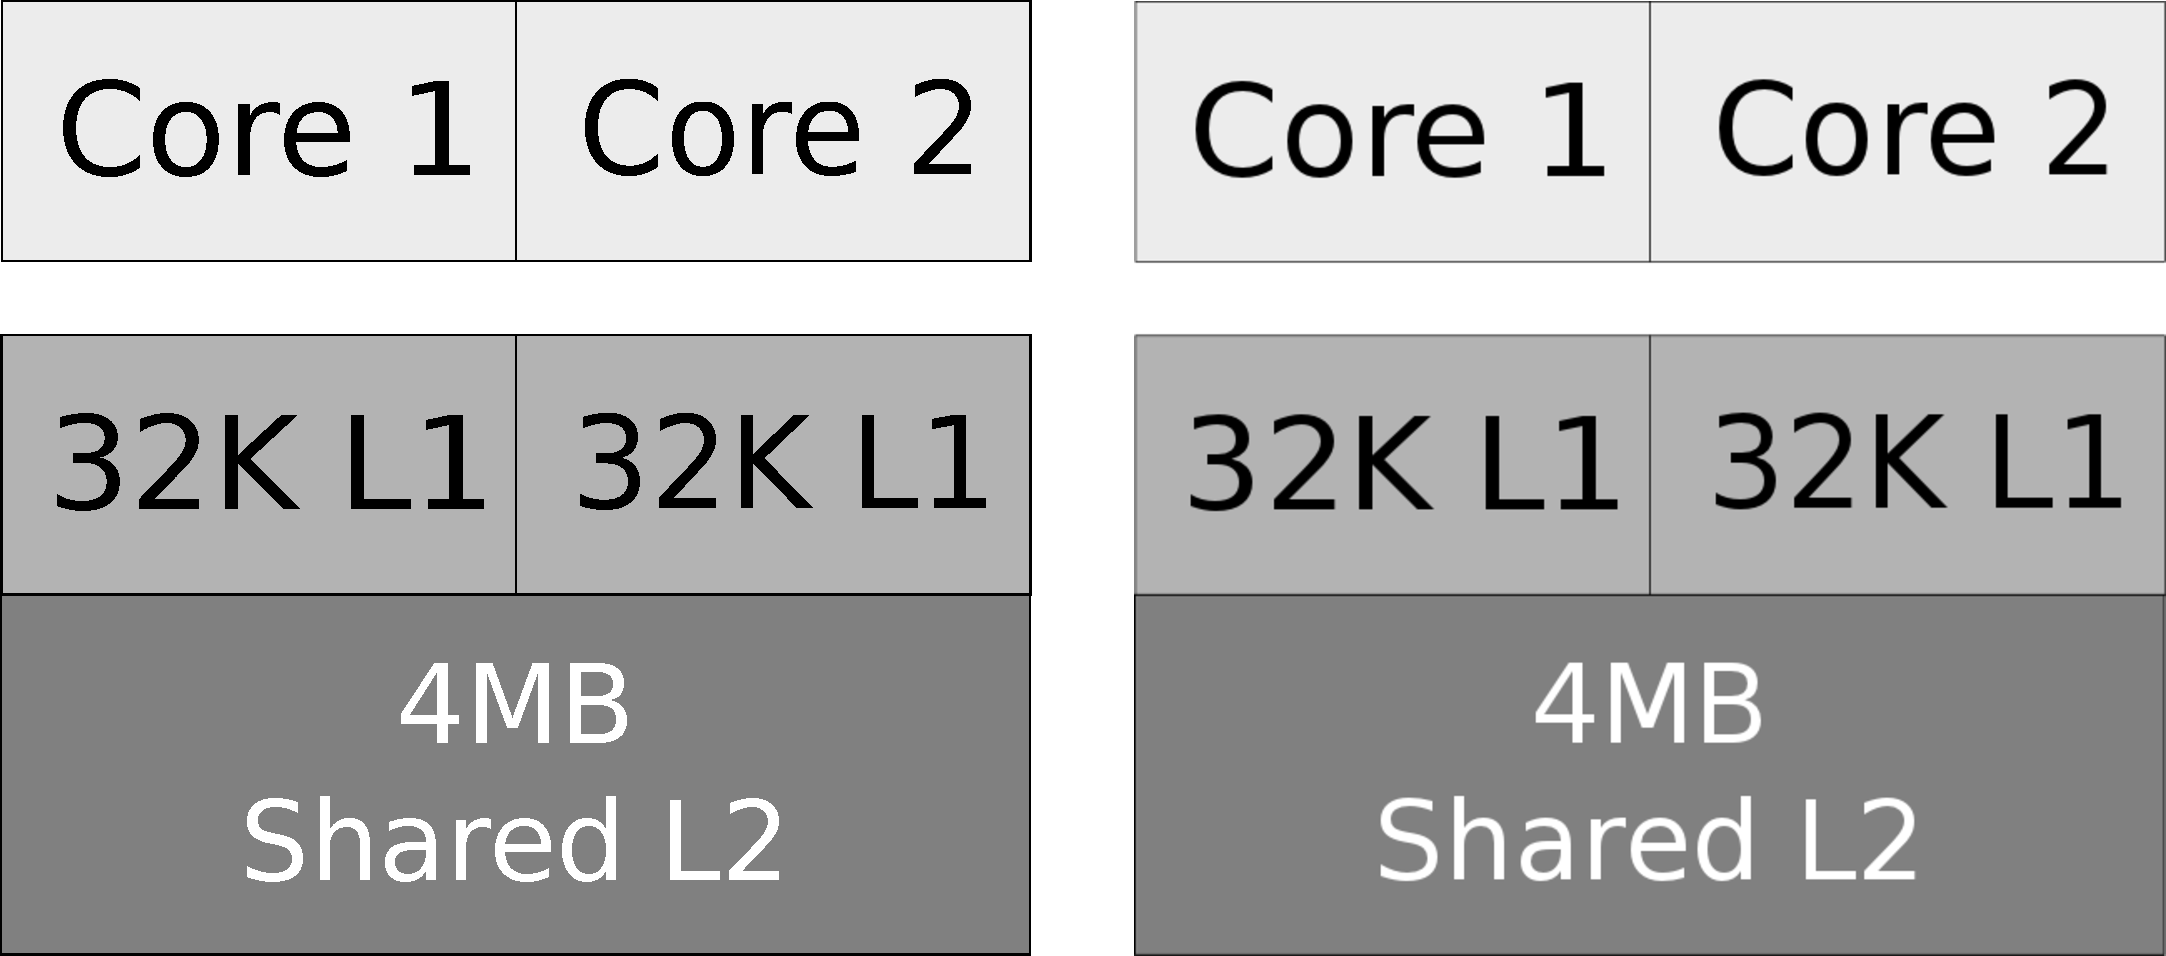
\includegraphics[width=0.5\textwidth]{xeon_die.pdf}
	\end{center}
	\caption{Architecture of the CPU}
\end{figure}

\begin{itemize}
	\item Intel Xeon E5354 @ 2.33GHz (\emph{Clovertown} processor)
	\begin{itemize}
		\item 2 \emph{Woodcrest} Core2 dies
		\item 2 sockets per chip
		\item Supports SSE, SSE2, SSSE3
	\end{itemize}
	\item Memory hierarchy
	\begin{itemize}
		\item $32$ KB Level 1 cache
		\item $4$ MB shared Level 2 cache
		\item $64$ byte cache line
		\item $16 \times 128$ bit SSE3 registers
	\end{itemize}
\end{itemize}

\subsection{Software}
\begin{itemize}
	\item CentOS 6.3 Linux (Kernel \texttt{2.6.32-358.18.1.el6.x86\_64})
	\item Built with GCC 4.7.3
	\item Compiler flags: \texttt{-foptimize-register-move -O3 -msse -funroll-loops -msse2 -msse3 -m3dnow -mfpmath=sse -mfpmath=sse -malign-double}
\end{itemize}

\section{Basic Algorithm}
The naive implementation of the matrix multiplication algorithm consists of three nested \lstinline{for} loops, where every loop runs from $1$ to $n$. In the innermost loop, a single addition and multiplication is done. Therefore, the runtime complexity of this algorithm is $\mathcal{O}(n^3)$ floating-point operations. We did not use an algorithm with a lower runtime complexity\footnote{Strassen's algorithm has a runtime complexity of $\mathcal{O}(n^{2.8})$.}.

\begin{figure}
\begin{lstlisting}
void square_dgemm (int n, double* A, double* B, double* C)
{
 	for (int i = 0; i < n; ++i)
    {
    	for (int j = 0; j < n; ++j)
    	{
			double cij = C[i*n+j];

			for (int k = 0; k < n; k++)
			{
				cij += A[i*n+k] * B[k*n+j];
				C[i*n+j] = cij;
    		}
    	}
    }
}
\end{lstlisting}
\caption{Naive matrix multiplication algorithm.}
\label{fig:naive_mul}
\end{figure}
Figure~\ref{fig:naive_mul} shows the basic matrix multiplication algorithm. We will reference this algorithm throughout the Section~\ref{sec:optim} and explain why our optimizations can increase the performance of the basic algorithm.

\section{Optimizations}\label{sec:optim}
In this section, we will describe and evaluation optimizations of our DGEMM algorithm.

\subsection{Blocking for L1 Cache}
To increase locality, we implemented blocking.  This restricts the computations into chunks that that fit inside the cache. In the basic algorithm, we read \lstinline{A} row by row left-to-right. \lstinline{B}, on the other hand, is read column by column from the top to the bottom. Every time we access a value in a matrix, we prefetch the next $7$ elements in that row\footnote{A cache line contains $8$ doubles.}, in case we have a cache miss.

%Main memory references are also decreased from $n^3+3n^2$ references in the naive implementation to $2*(n+2)*n^2$. The flop to memory ratio, $q$, is also drastically reduced from $q=2$ as n $\rightarrow \infty$ to $q=n/N=\mathit{BLOCK\_SIZE}$ as n $\rightarrow \infty$.  As the flop to memory ratio decreases, so does the number of caches misses. There are $(n^2_B/8 + n^2_B/8)(n/\mathit{BLOCK\_SIZE})$ cache misses for every C block computed, multiplied by $(N/\mathit{BLOCK\_SIZE})^2$ blocks in C, for a total of $N^3/(4N_B)$. , compared to $(9/8)N^3$.

\begin{lstlisting}
for (int i = 0; i < BLOCK_SIZE; i++)
	for (int j = 0; j < BLOCK_SIZE; j++)
		for (int k = 0; k < BLOCK_SIZE; k++)
			C[i][j]+=A[i][k]+B[k][j];
\end{lstlisting}

\subsection{Blocking for L2 Cache}
The size of the Level 2 cache is $4$ MB. Therefore, we can store $\frac{4 \cdot 1024^2}{8}$ matrix entries in the L2 cache. Since we have three matrices \lstinline{A}, \lstinline{B}, and \lstinline{C}, blocking for the L2 cache can increase the performance only if $n > \sqrt{\frac{4 \cdot 1024^2}{8 \cdot 3}} = 418$. In our benchmarks, we did not deal with matrices bigger than $1200$ entries. Therefore, we do no blocking for the L2 cache in our final implementation. We implemented L2 blocking in an intermediate version and it lead to a performance decrease, especially for small matrix sizes.
% theoretical explanation why it does not work

\subsection{Matrix Transposition}

\subsection{Register Blocking and Loop Unrolling}

\subsection{Matrix Buffering}

\subsection{Streaming SIMD Extensions (SSE)}
% + fused add multiply

\subsection{Parameter Tuning}
Parameter tuning is the task of trying (brute-force) a set of parameters that affect the performance.

\subsubsection{Motivation}
As shown before, for certain matrix sizes $n$, the blocked algorithm performes better with certain block sizes. One obvious reason is that for a fixed matrix size $n$, the block size determines the size of the fringe cases. The code for fringe cases is less optimized than the code for regular cases and fringe cases might take less advantage of the cache. Also remember, that a cache line is $64$ bytes long and the size of a fringe case might not be divisible by the cache line size, i.e. a cache line is eventually not filled entirely with data from the fringe case. Therefore, we want to keep the fringe cases as small as possible. Let $f_i$ be the size of the fringe cases in dimension $i$\footnote{The same argument applies for the other dimensions.}. 

$$f_i = n \mod b_i$$

For example, for $n=372$, $b_i=16$ might be a better block size than $b_i=32$, because it results in fringe cases of size $4$ instead of $20$.

\subsubsection{Search Space}
We tried values for $b_i$, $b_j$ and $b_k$ for the L1 cache blocking. Due to certain implementation details, $b_i$ and $b_j$ must always be the same value. A cache line is $64$ bytes ($8$ doubles) long. Therefore, in order to reduce the search space, it makes sense to only take a look at multiples of $8$. We tried all possible combinations of $b_i=b_j, b_k \in \{8, 16, 24, 32, 40, 48, 56, 64\}$, resulting in $64$ parameter combinations. We ran the program for every matrix size from $n=10$ to $n=1200$. For every value of $n$, we then selected the parameters $b_i$ and $b_k$ with the highest performance. 

\subsubsection{Implementation}
We hard-coded the block size parameters for all matrix sizes from $n=10$ to $n=1200$. Based on the matrix size, a different version of the algorithm with the respective block size is run. For all other matrix sizes, we use $b_i=b_j=8$, $b_k=64$, because it performed good on average.

\subsubsection{Results and Evaluation}
Figure~\ref{fig:param_results} shows the performance of the parameter-tuned version of our implementation. It is interesting to see, that for some very small matrix sizes, our implementation is faster than ATLAS. The Appendix contains some more graphs without parameter tuning, but for fixed block sizes. We can observe that the performance of the algorithm reaches a peak when the matrix size is a multiple of one or two of block sizes. In that case, we have no fringe cases.
\begin{figure}
	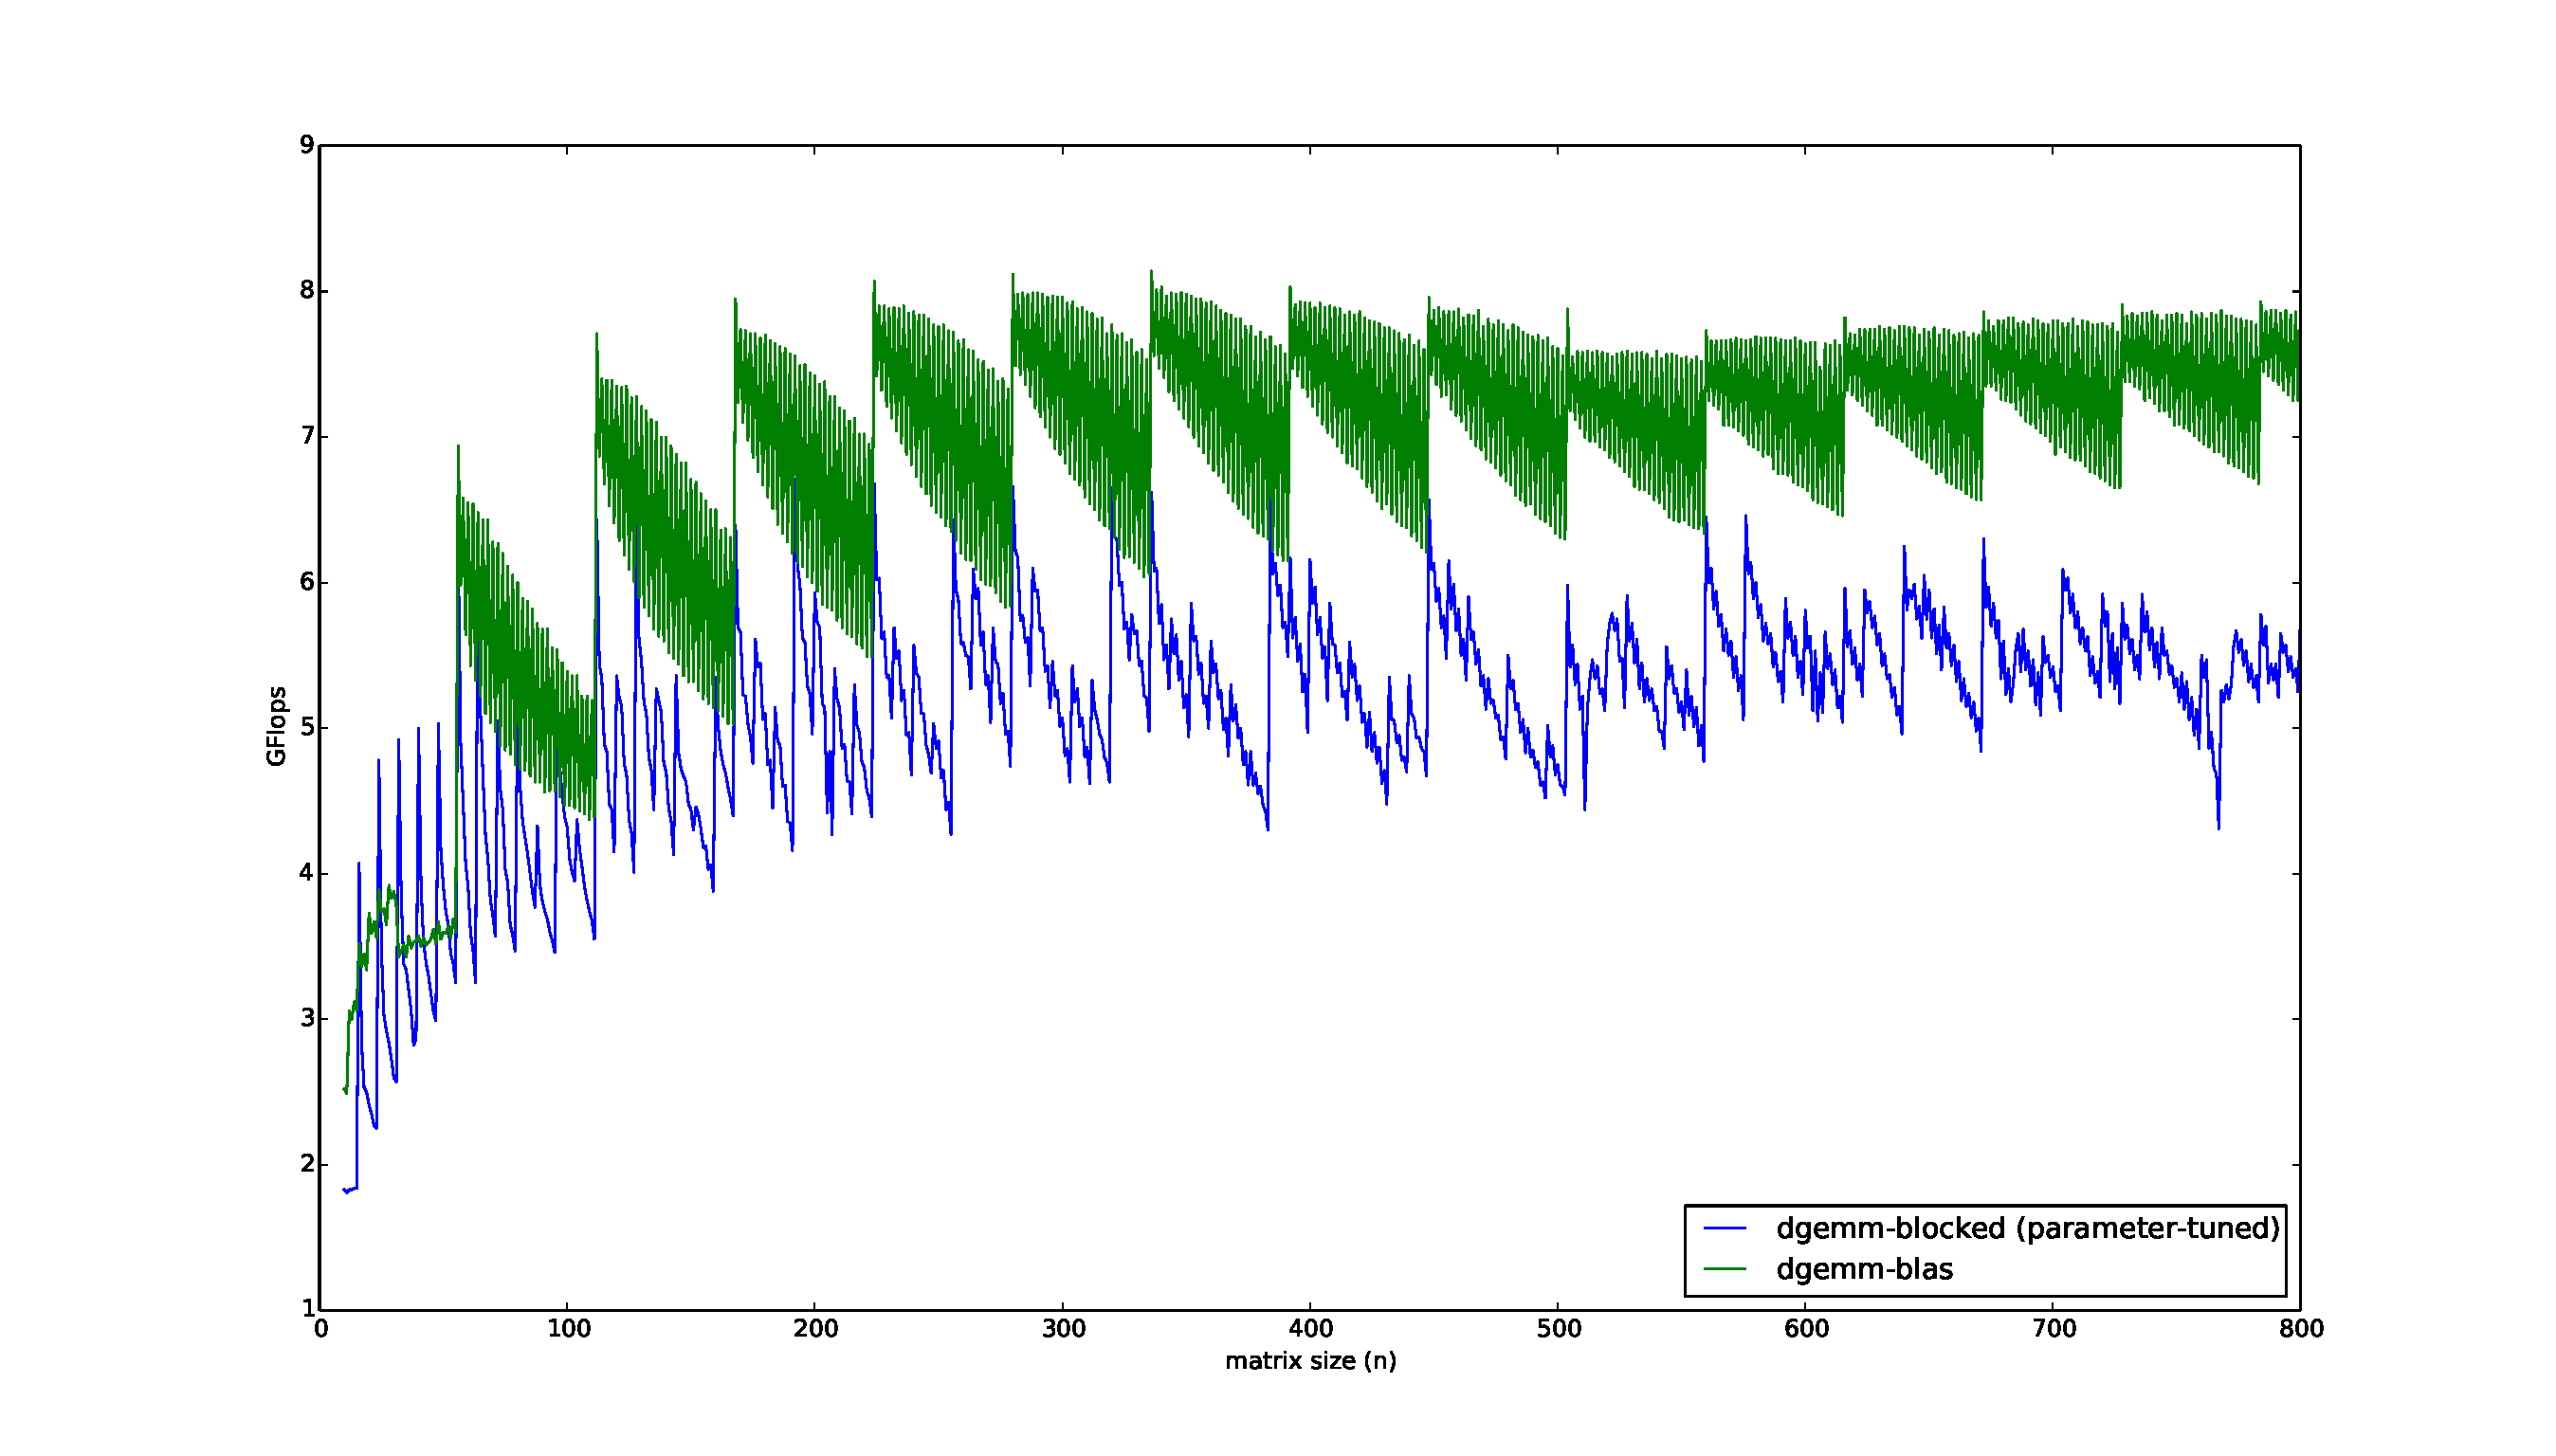
\includegraphics[width=\textwidth]{graphs/profiles/PROFILE_BLOCKED.pdf}
	\caption{Performance of our parameter-tuned blocking version, in comparison to ATLAS.}
	\label{fig:param_results}
\end{figure}

\section{Performance Evaluation}
\subsection{Parameter Tuning}

\newpage
\section*{Appendix}
\subsection*{Performance Tuning}
%\begin{tabular}{cccc}
	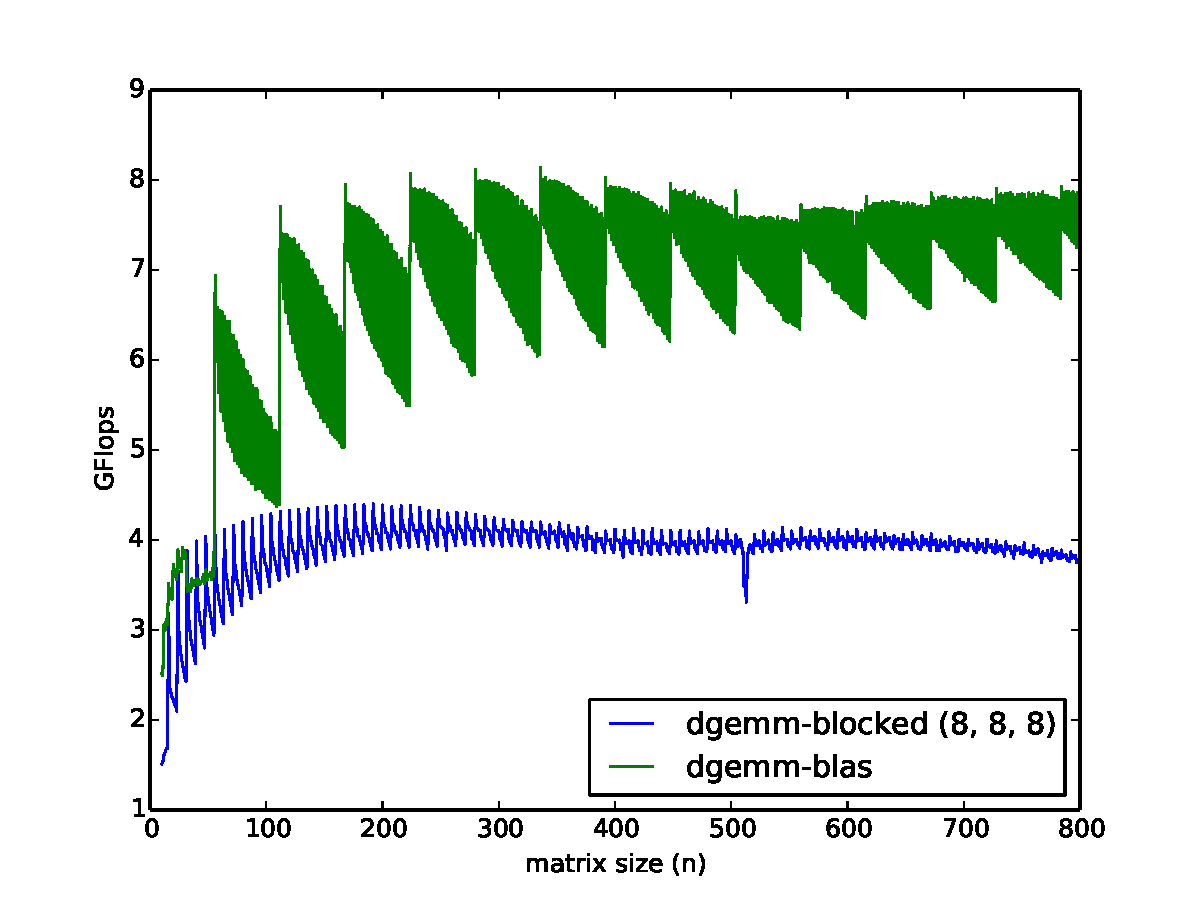
\includegraphics[width=0.25\textwidth]{graphs/profiles/PROFILE_OUTUT_8_8.pdf}  
	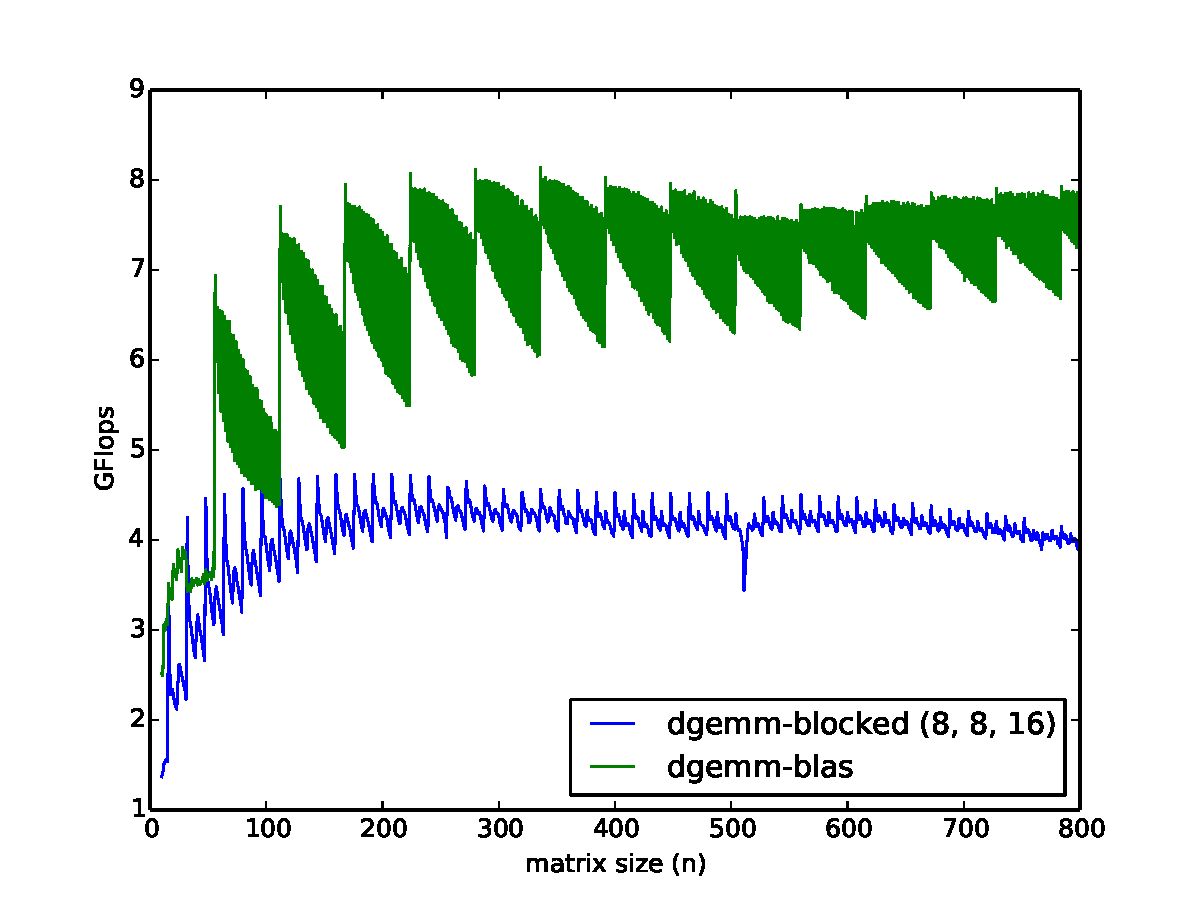
\includegraphics[width=0.25\textwidth]{graphs/profiles/PROFILE_OUTUT_8_16.pdf}  
	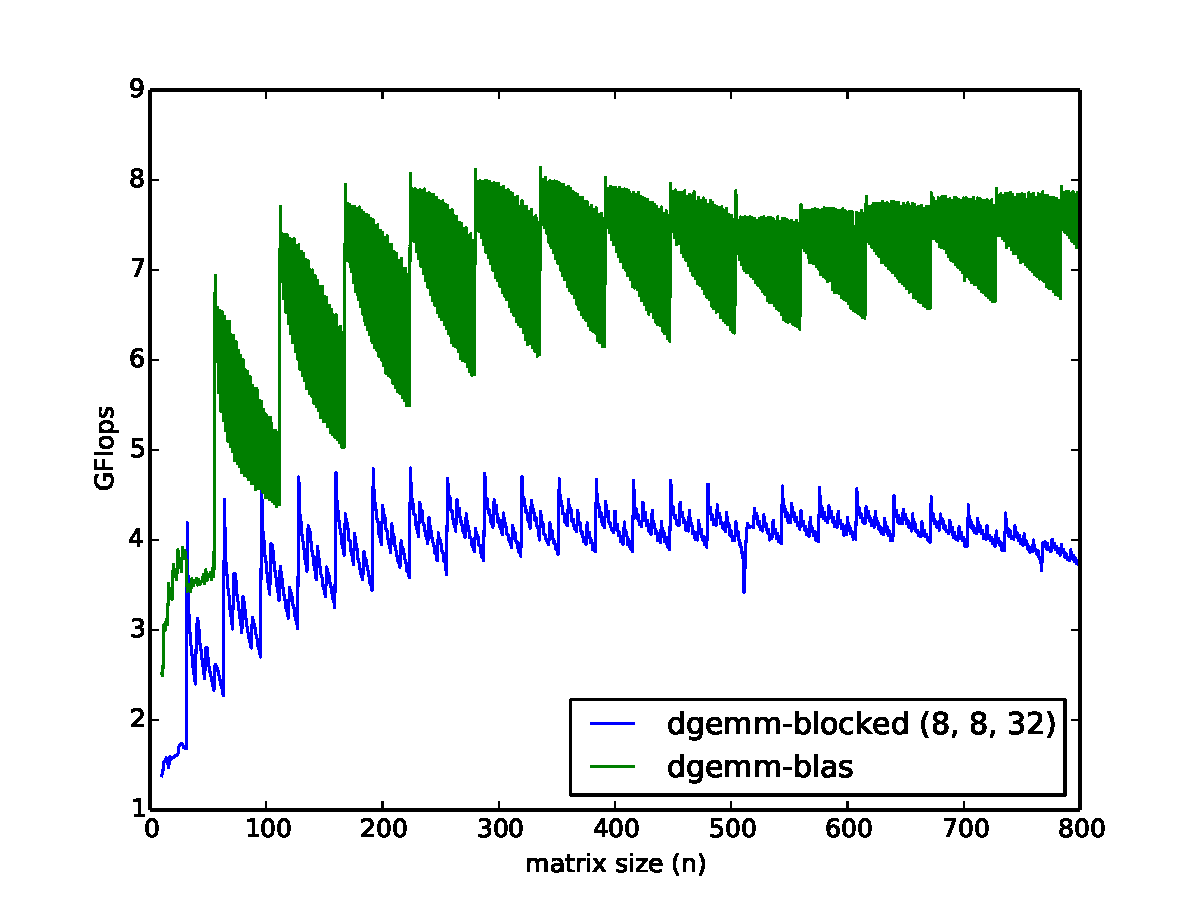
\includegraphics[width=0.25\textwidth]{graphs/profiles/PROFILE_OUTUT_8_32.pdf} 
	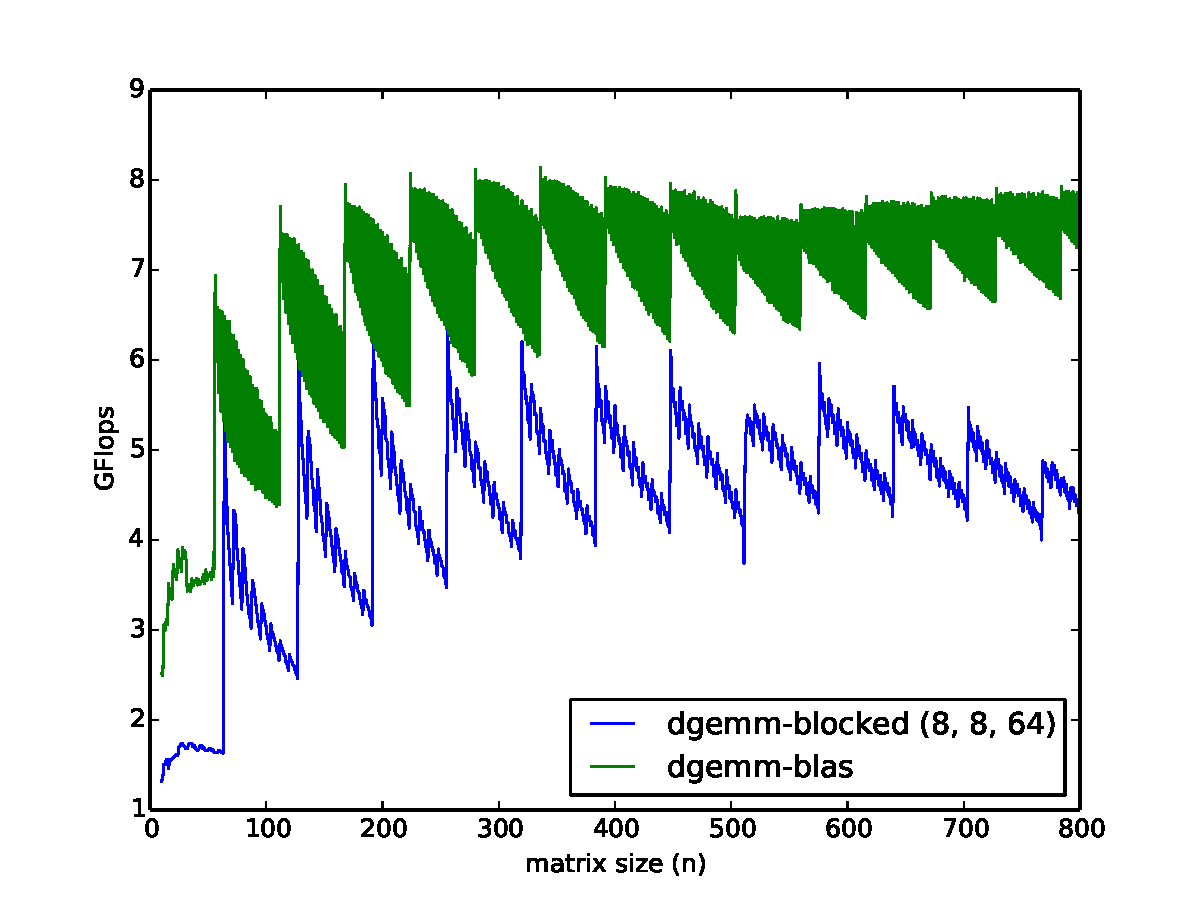
\includegraphics[width=0.25\textwidth]{graphs/profiles/PROFILE_OUTUT_8_64.pdf} 
	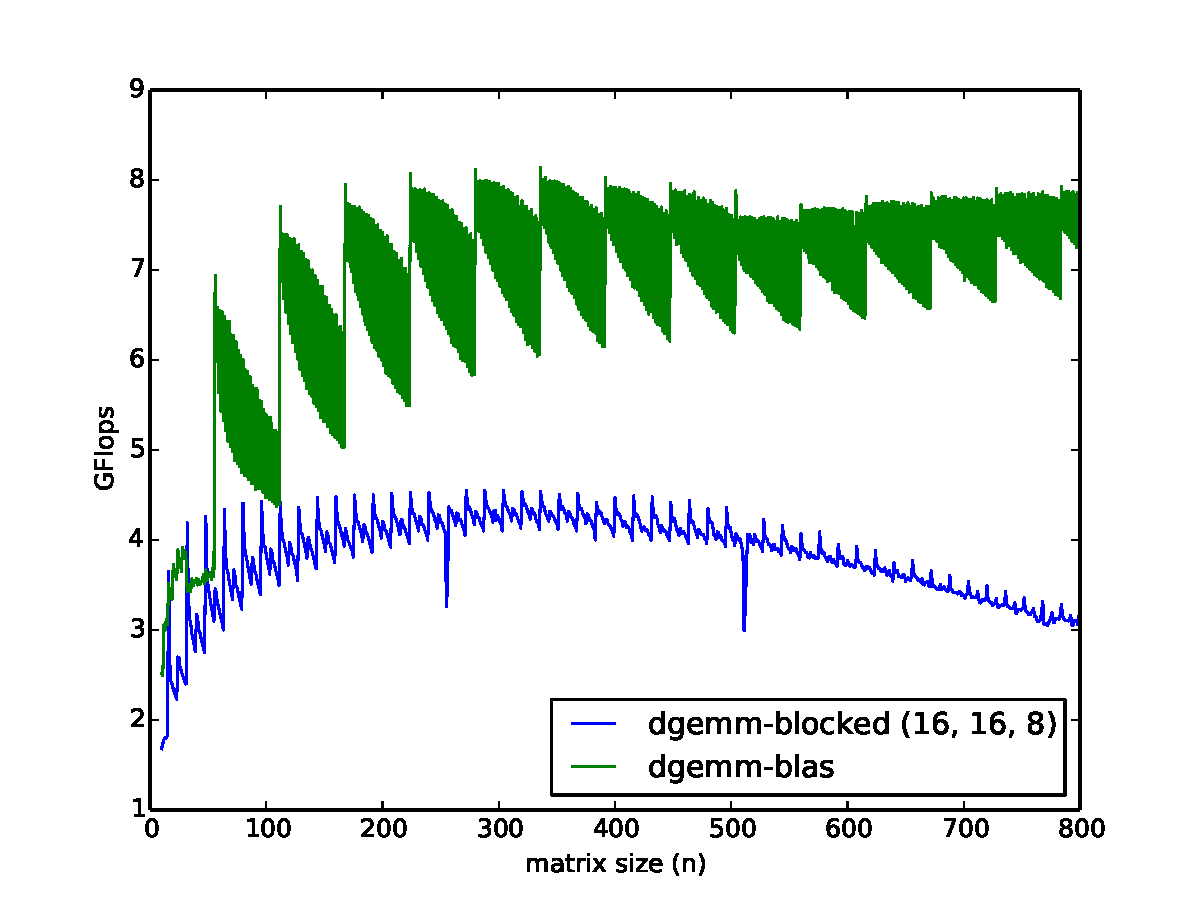
\includegraphics[width=0.25\textwidth]{graphs/profiles/PROFILE_OUTUT_16_8.pdf}  
	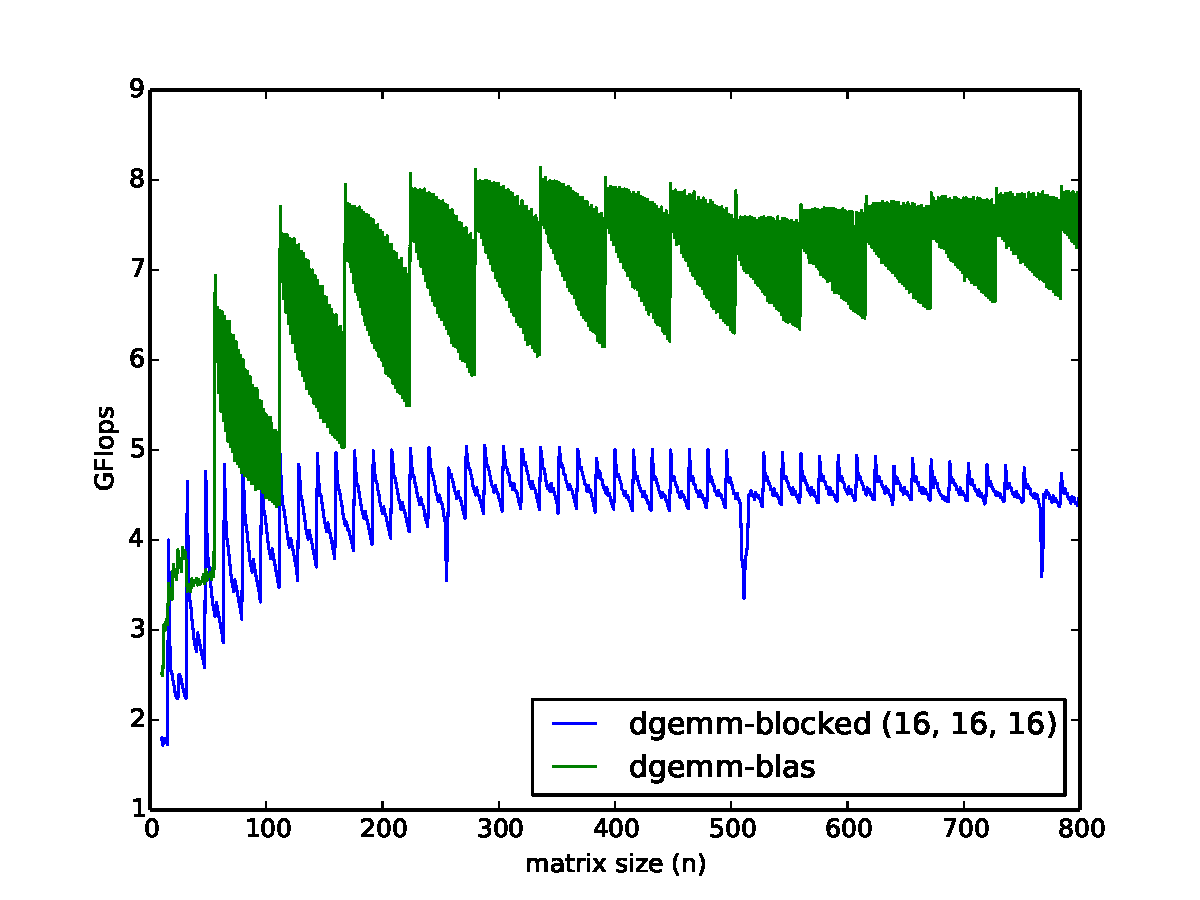
\includegraphics[width=0.25\textwidth]{graphs/profiles/PROFILE_OUTUT_16_16.pdf}  
	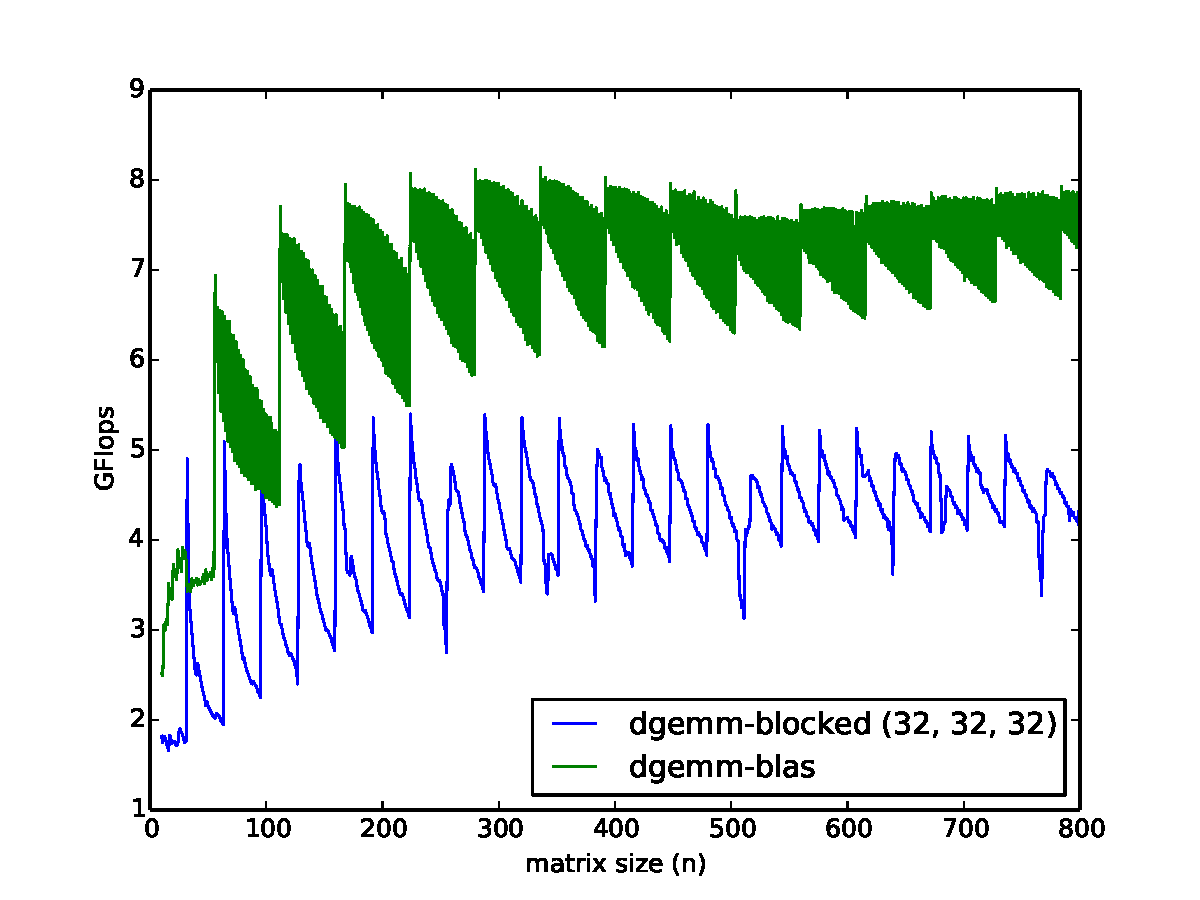
\includegraphics[width=0.25\textwidth]{graphs/profiles/PROFILE_OUTUT_32_32.pdf} 
	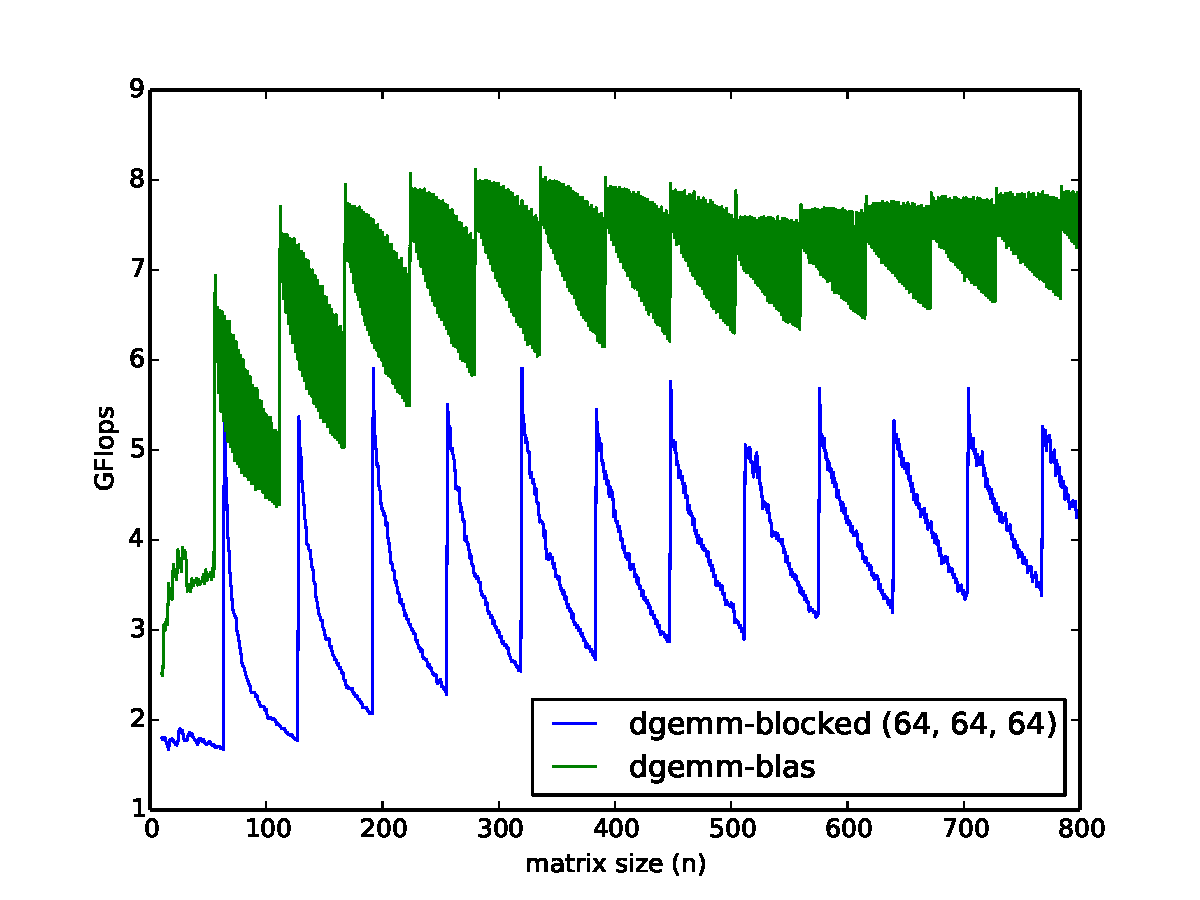
\includegraphics[width=0.25\textwidth]{graphs/profiles/PROFILE_OUTUT_64_64.pdf} 
	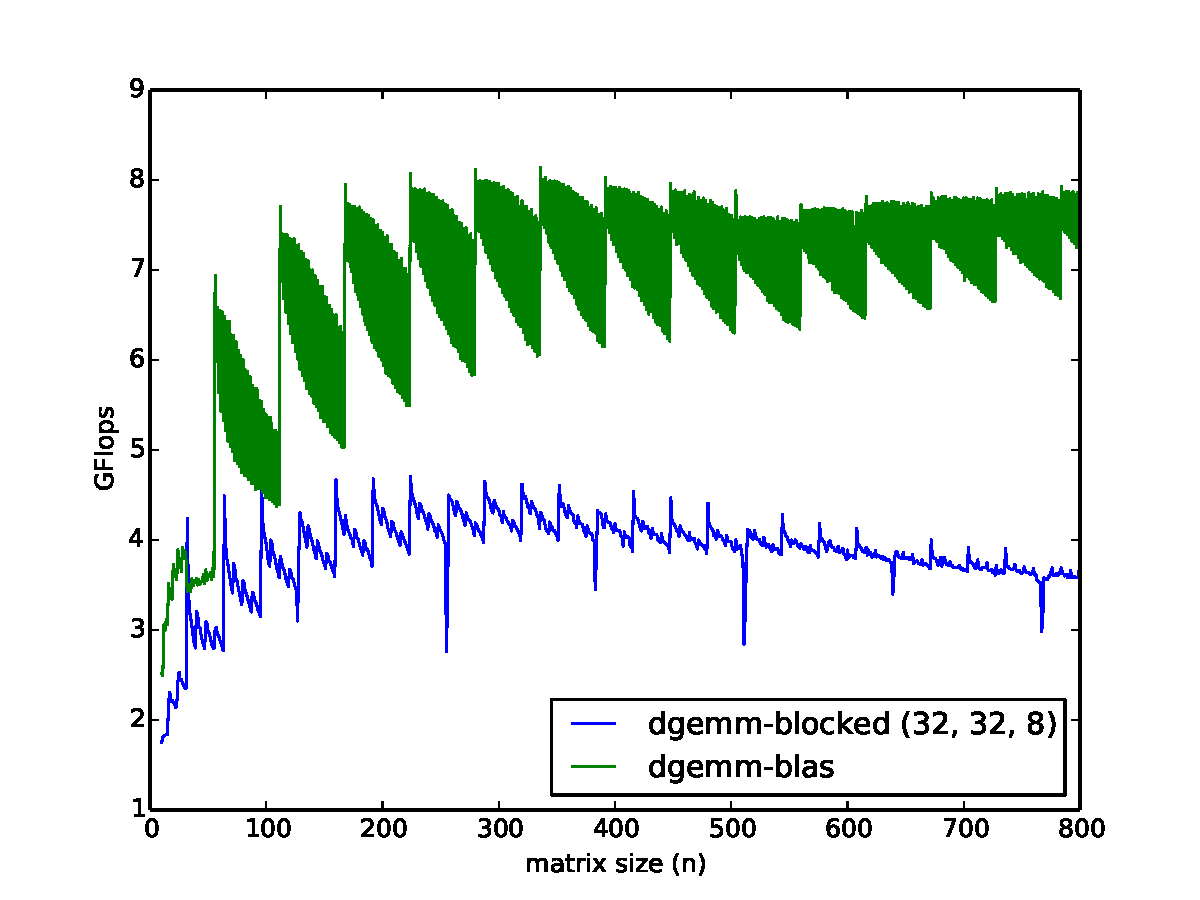
\includegraphics[width=0.25\textwidth]{graphs/profiles/PROFILE_OUTUT_32_8.pdf}  
	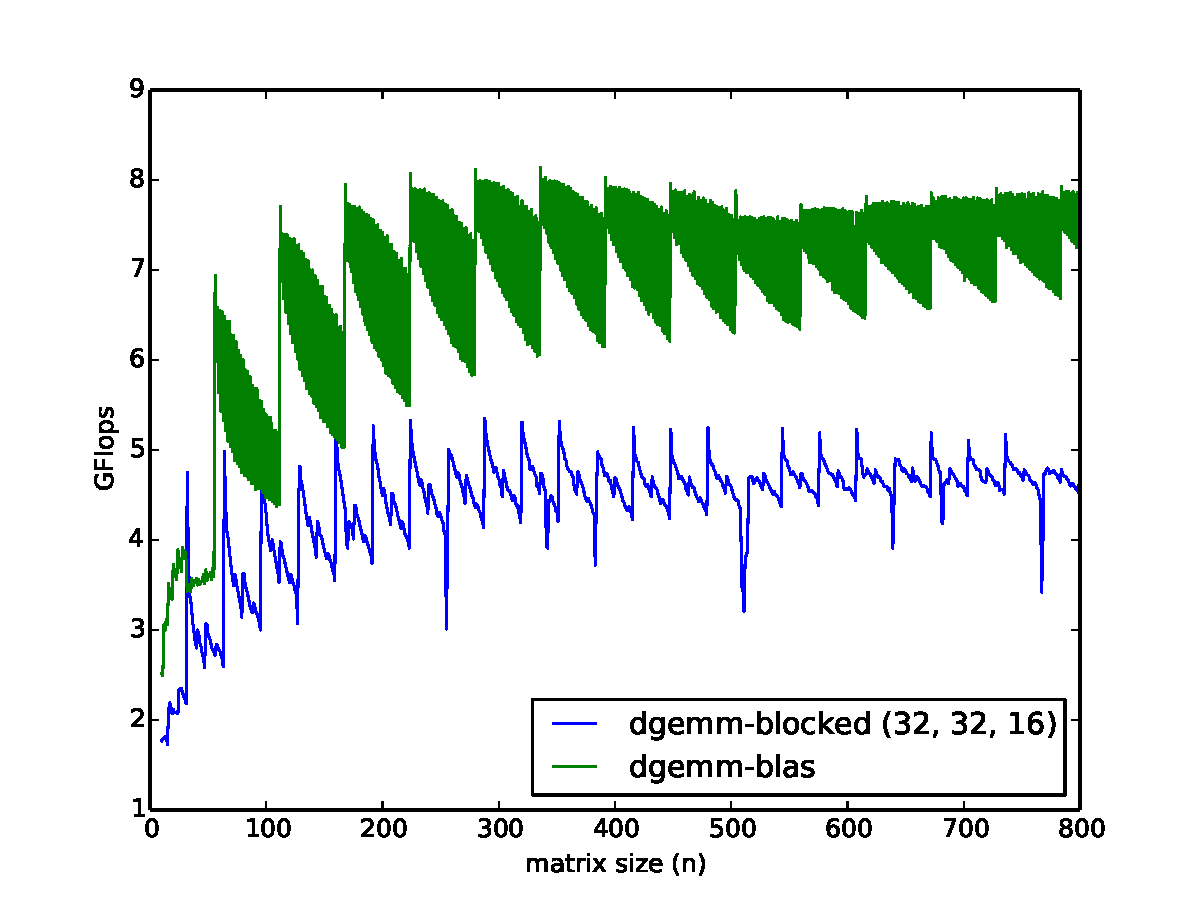
\includegraphics[width=0.25\textwidth]{graphs/profiles/PROFILE_OUTUT_32_16.pdf}  
	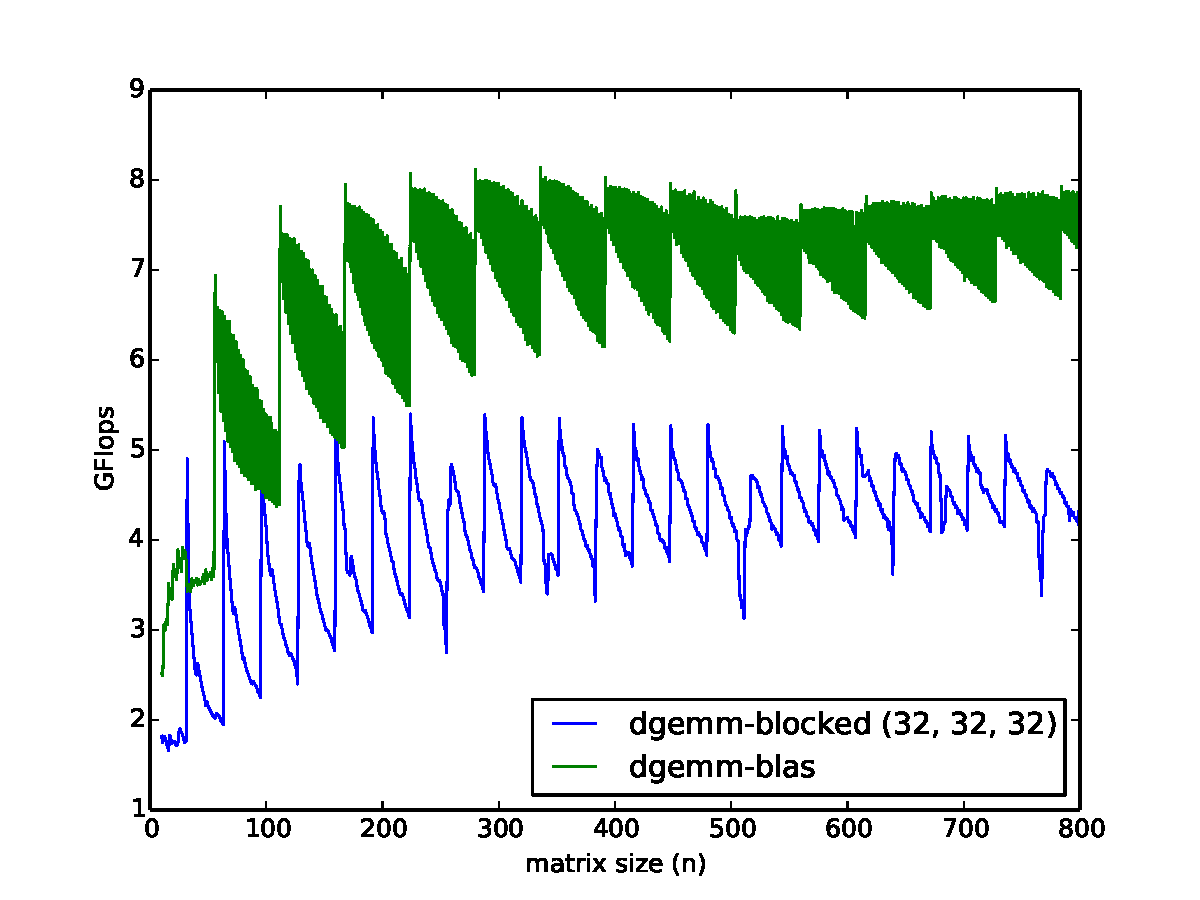
\includegraphics[width=0.25\textwidth]{graphs/profiles/PROFILE_OUTUT_32_32.pdf} 
	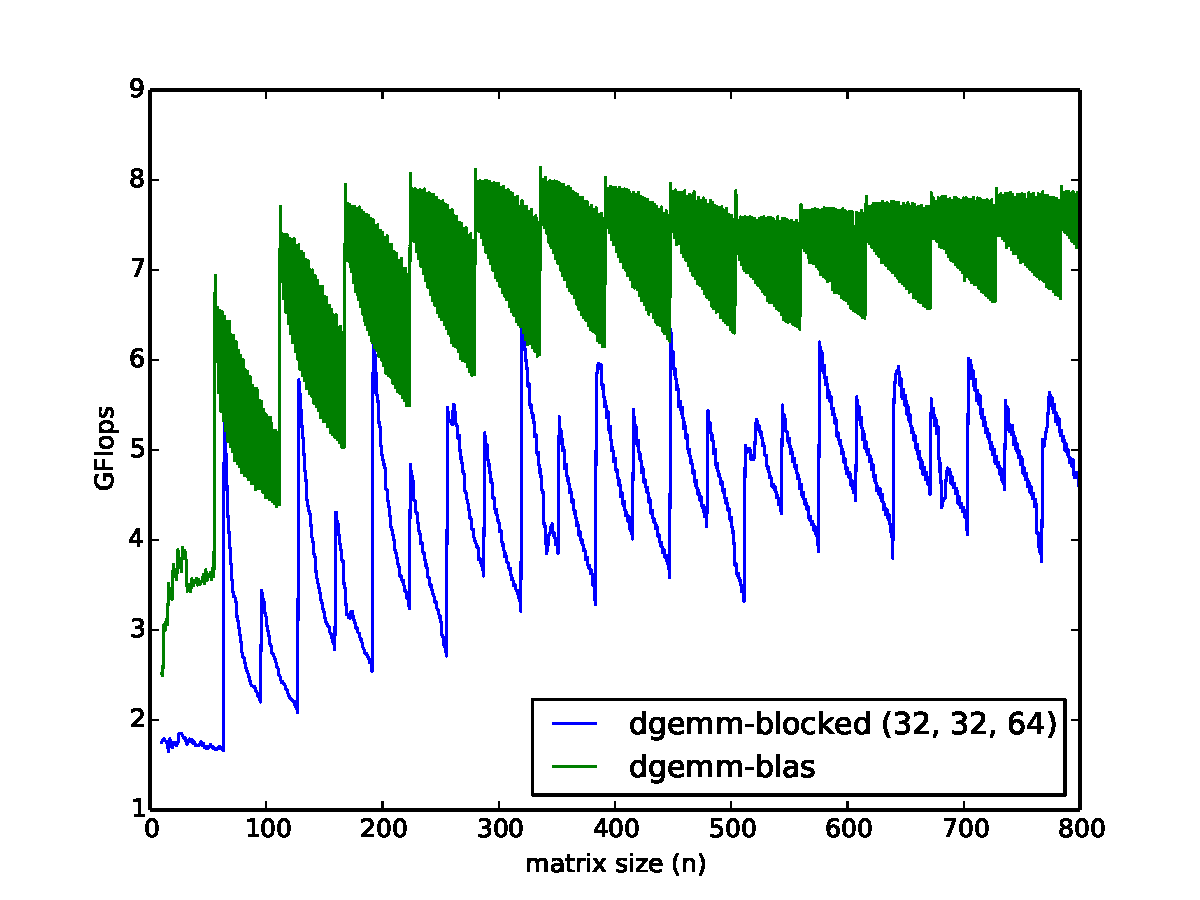
\includegraphics[width=0.25\textwidth]{graphs/profiles/PROFILE_OUTUT_32_64.pdf} 
	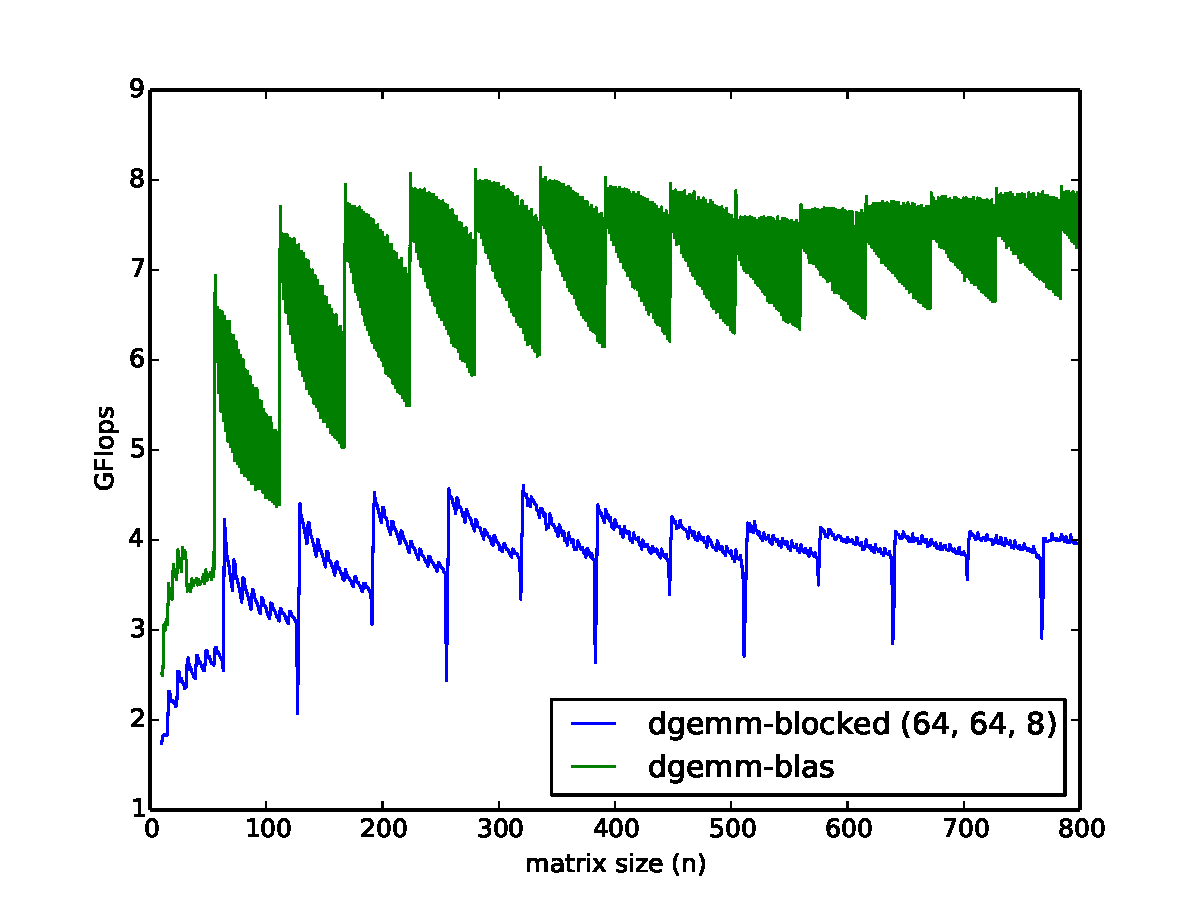
\includegraphics[width=0.25\textwidth]{graphs/profiles/PROFILE_OUTUT_64_8.pdf}  
	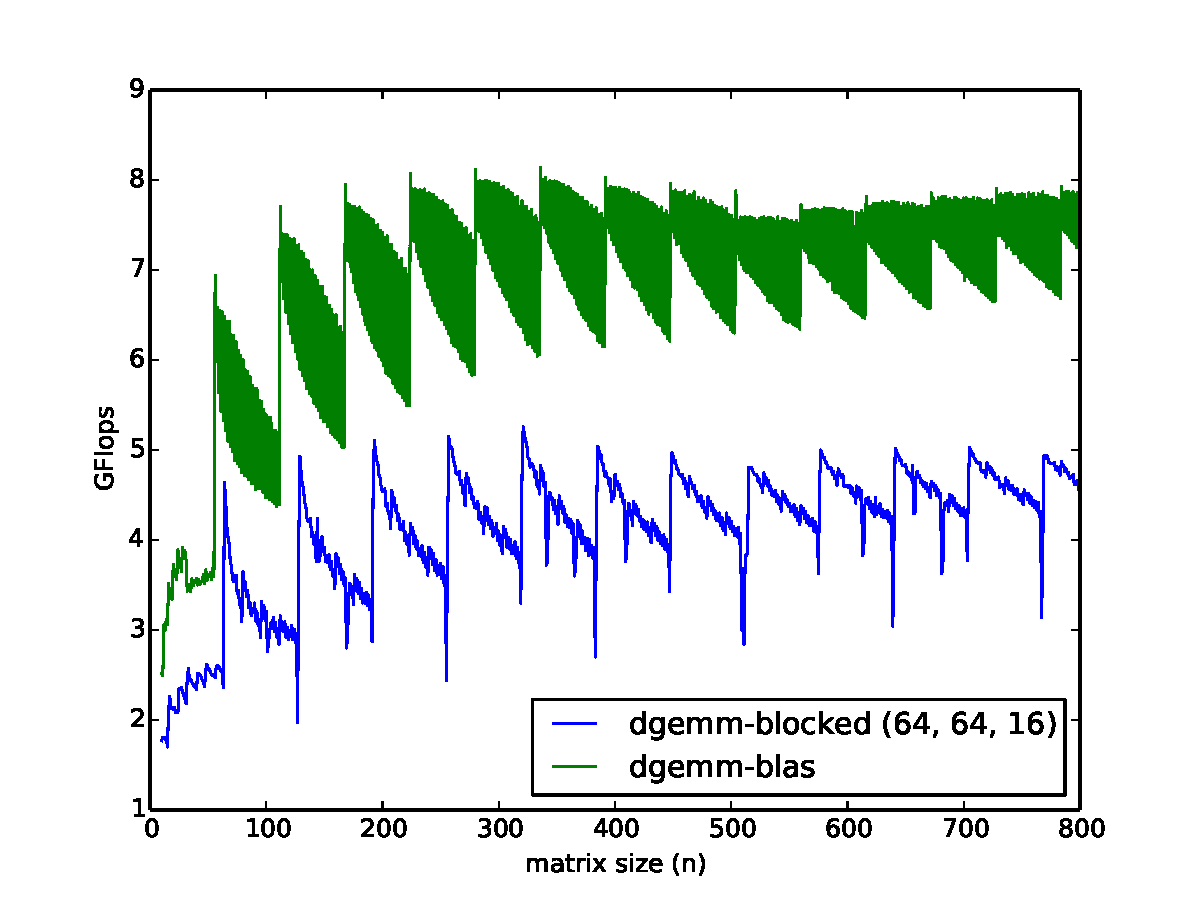
\includegraphics[width=0.25\textwidth]{graphs/profiles/PROFILE_OUTUT_64_16.pdf}  
	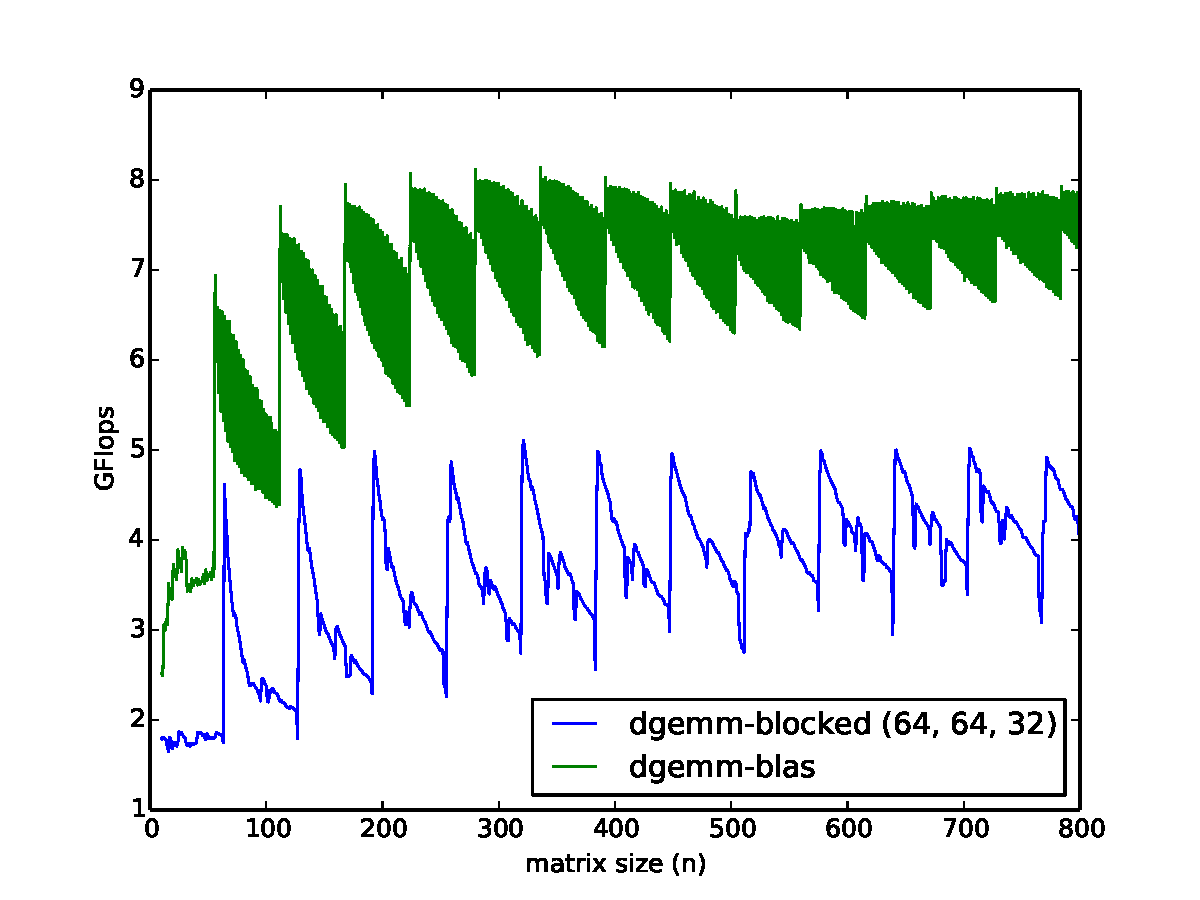
\includegraphics[width=0.25\textwidth]{graphs/profiles/PROFILE_OUTUT_64_32.pdf} 
	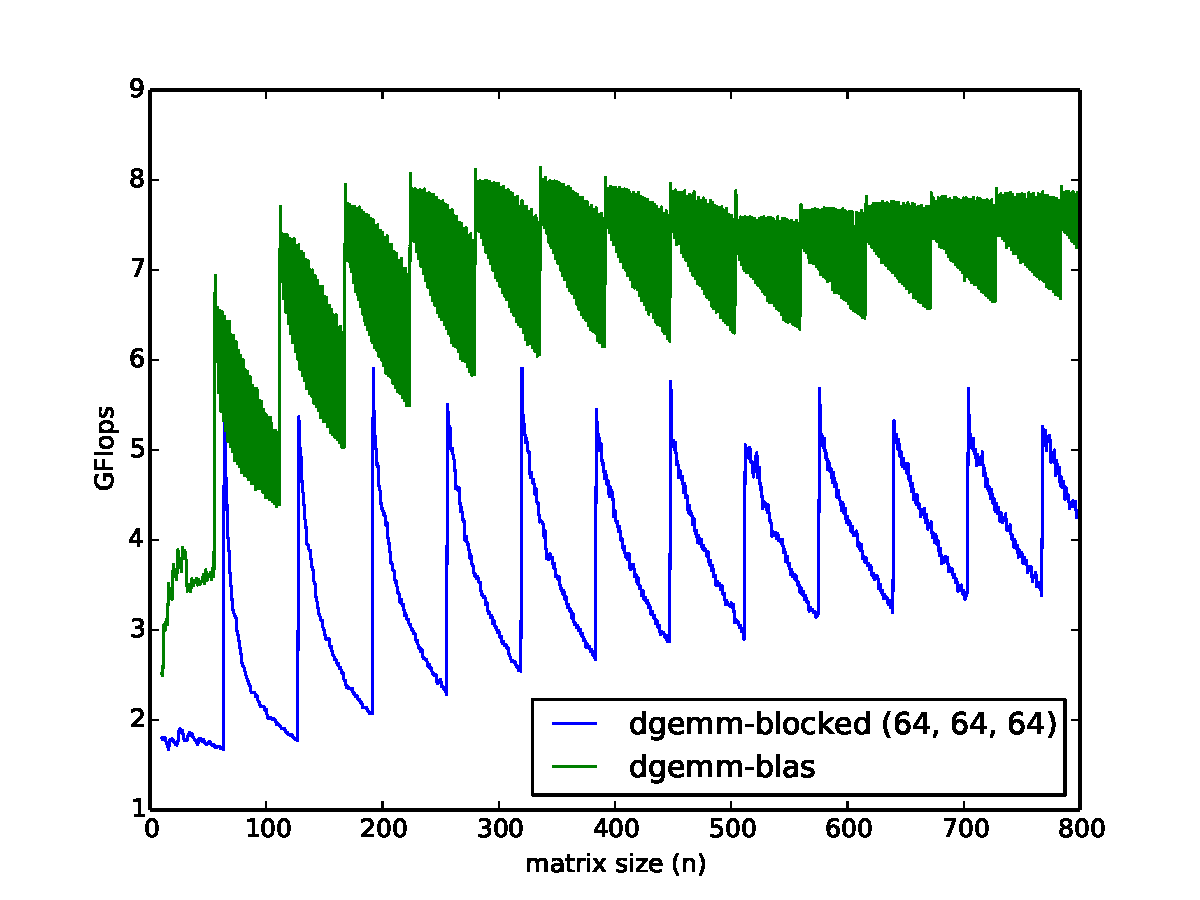
\includegraphics[width=0.25\textwidth]{graphs/profiles/PROFILE_OUTUT_64_64.pdf} 
	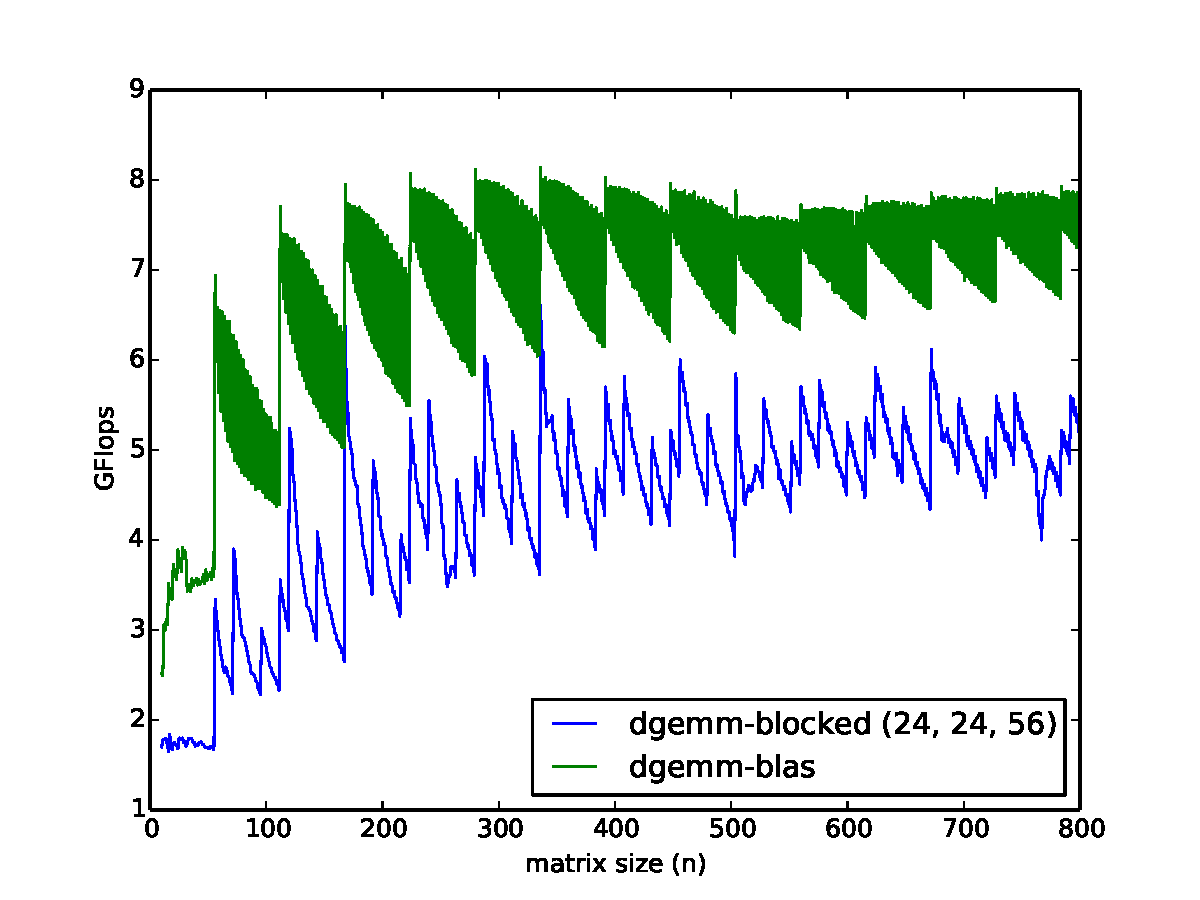
\includegraphics[width=0.25\textwidth]{graphs/profiles/PROFILE_OUTUT_24_56.pdf}  
	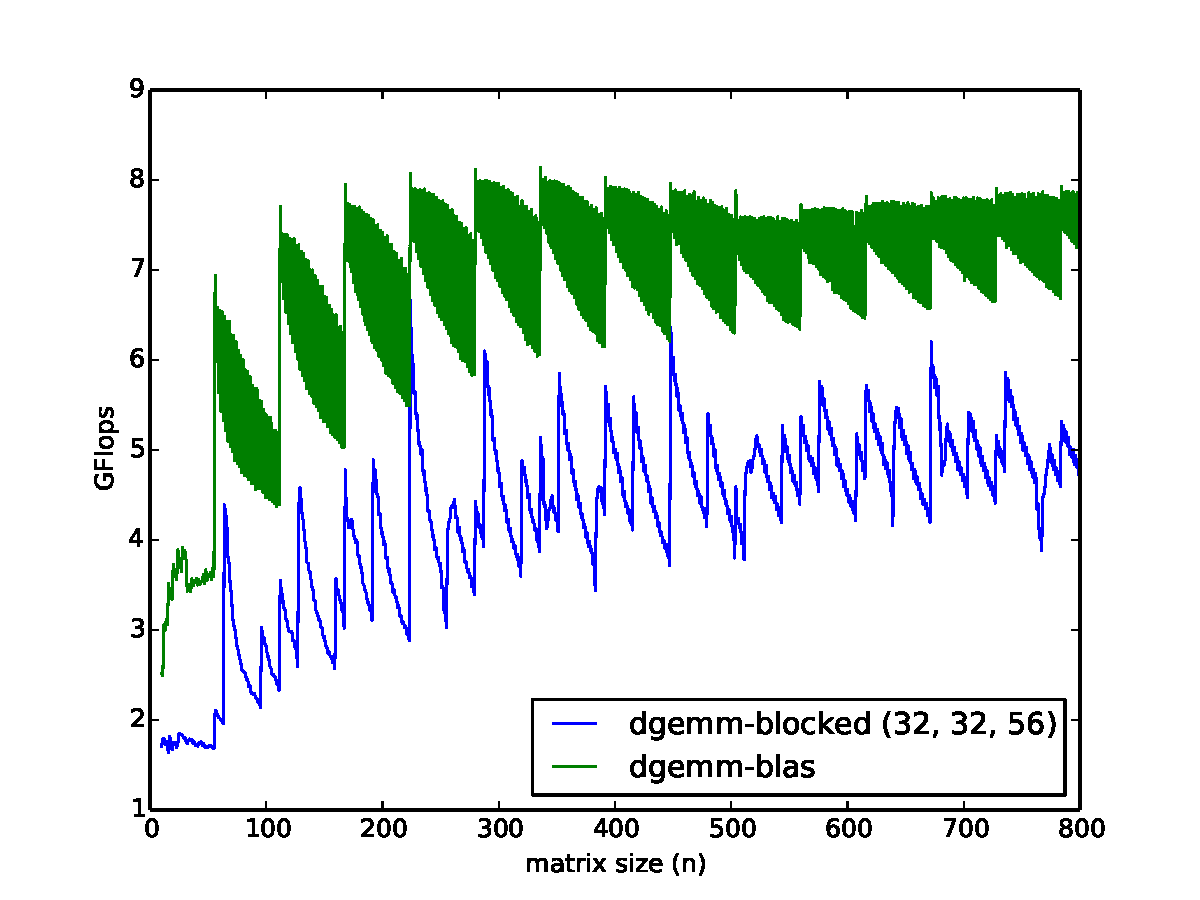
\includegraphics[width=0.25\textwidth]{graphs/profiles/PROFILE_OUTUT_32_56.pdf}  
	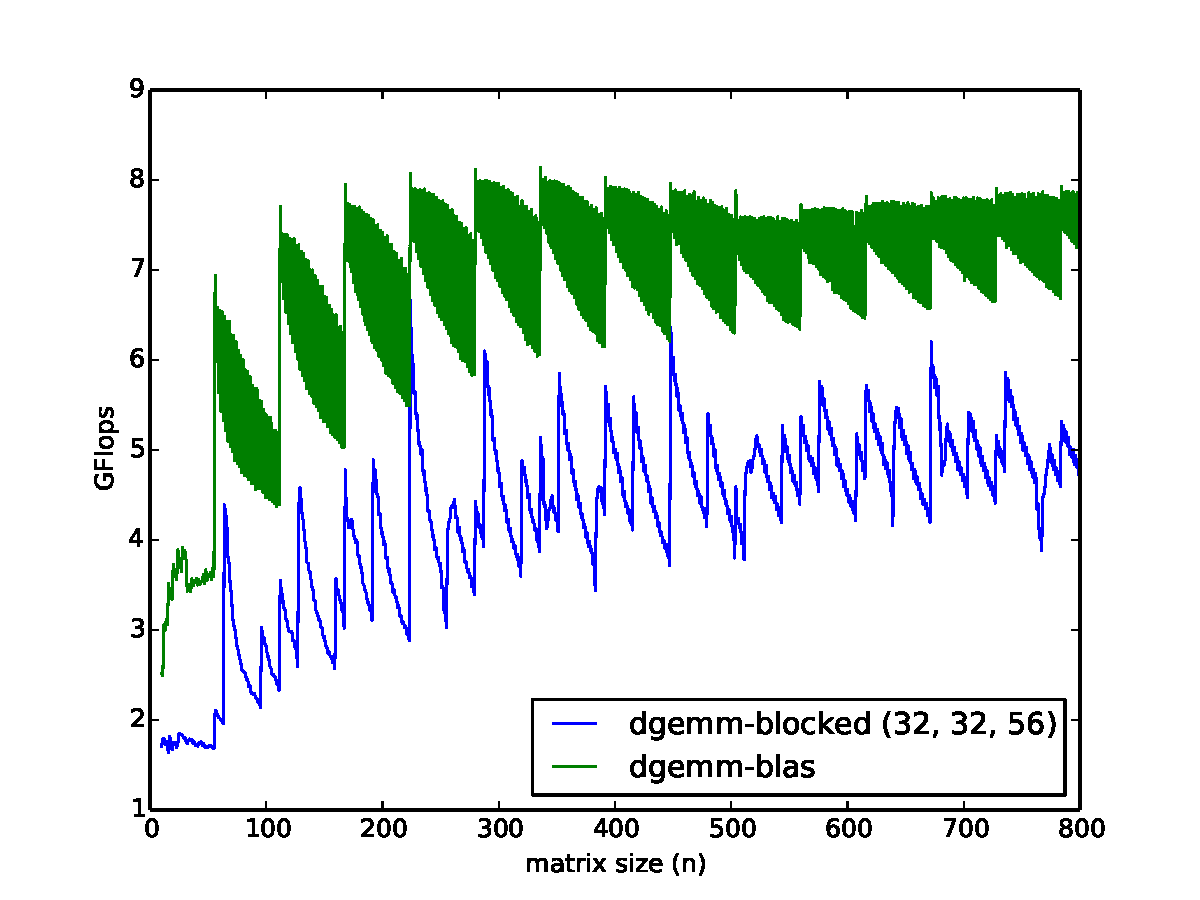
\includegraphics[width=0.25\textwidth]{graphs/profiles/PROFILE_OUTUT_32_56.pdf} 
	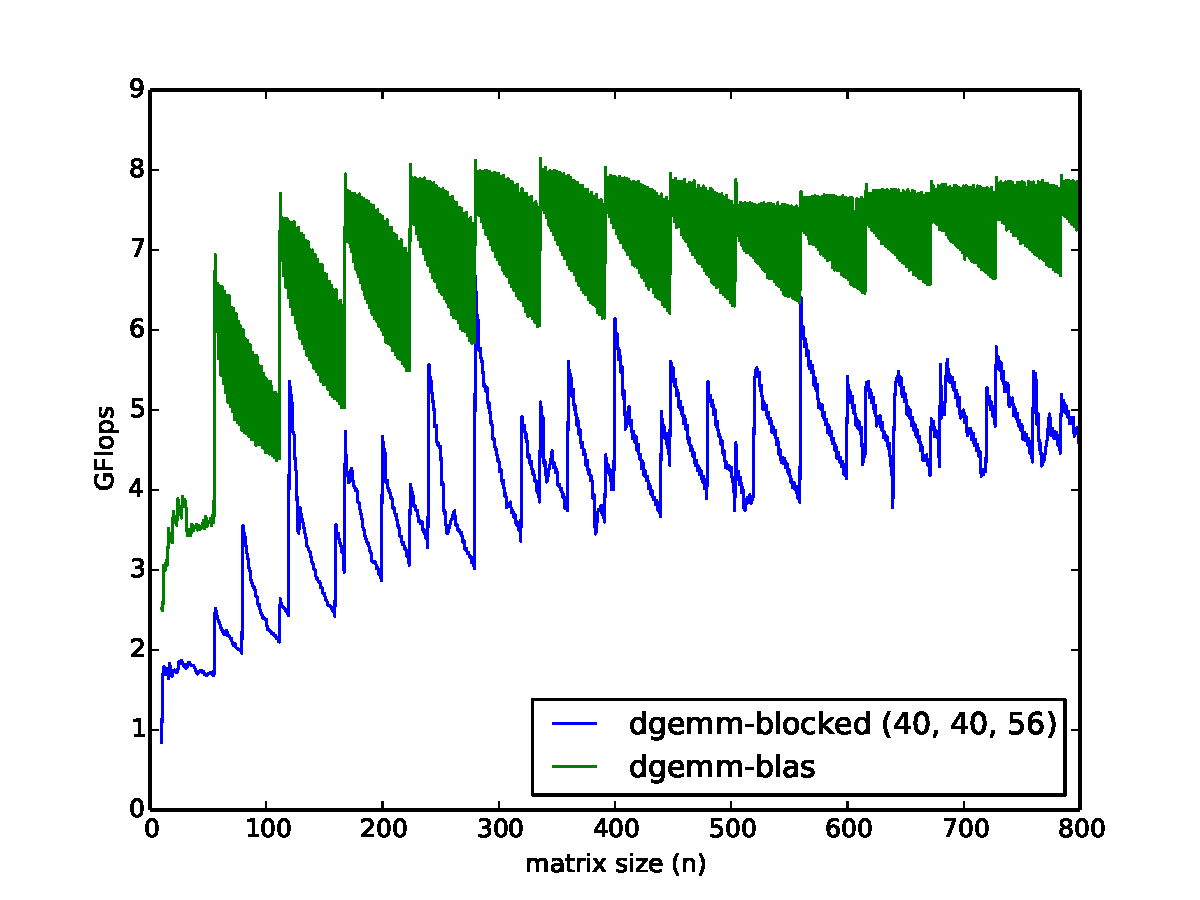
\includegraphics[width=0.25\textwidth]{graphs/profiles/PROFILE_OUTUT_40_56.pdf} 
%\end{tabular}
\end{document}

